%==================================================
% Plantilla elaborado por Dr. David Pareja Quispe
% e-mail: dparejaq@unmsm.edu.pe
% No eliminar los créditos del Autor
%================================================
\documentclass[twoside,onehalfspace]{unmsmtesis}
%%   oneside          - hojas impresas por un solo lado
%%   twoside (*)      - hojas impresas por ambos lados

%=================================================
% ADICIONAR OTROS PAQUETES SI ES NECESARIO
%====================================================
\graphicspath{{Figuras/}}%Ruta de las figuras
\usepackage{blindtext}




%==========================================
%    Fuente
%==========================================
\newcommand*{\captionsource}[2]{%
  \caption[{#1}]{#1}\smallskip\par
  \textbf{Fuente:} #2\par}
  
%====================================================================
% Otra forma de colocar la fuente a las figuras de otros autores.
%====================================================================
\usepackage{copyrightbox} % Está dedicado a las notas de las imágenes situadas debajo, izquierda o a la derecha de las imágenes
\makeatletter
\renewcommand{\CRB@setcopyrightfont}{%
\footnotesize %Cambiar el tamanho de fuente 
\color{black} %Comentar si desea en el color por defecto
%\sc
}

%%%%%%%%%%%%%%%%%%%%%%%%%%%%%%%%%%%%%%%%%%%%%%%%%%%%%%%%%%%%%
%%%%%%%%%%%%%% AQUÍ INICIA EL DOCUMENTO %%%%%%%%%%%%%%%%%%%%%
%%%%%%%%%%%%%%%%%%%%%%%%%%%%%%%%%%%%%%%%%%%%%%%%%%%%%%%%%%%%%
%\setlength {\marginparwidth}{2cm} 
\begin{document}

%%%%%%%%%%%%%%%%%%%%%%%%%%%%%%%%%%%%%%%%%%
% CARGANDO LA PORTADA DEL DOCUMENTO
\begin{titlepage}
	\centering
	\vspace{-20pt}
    \hrule {\color{purple} \rule{\linewidth}{0.5mm}} \hrule 
    %\vspace{0.05cm}
    %\hrule
	\vspace{0.8cm}
	\textsc{\Large \textbf{Universidad Nacional Mayor San Marcos}\\}
	\vspace{0.5cm}
	\textbf{\normalsize Universidad del Perú, DECANA DE AMÉRICA\\}
    \vspace*{0.8cm}
    \hrule  {\color{purple} \rule{\linewidth}{0.5mm}} \hrule
	\vspace{1.2cm}
	\textsc{\Large \bfseries Facultad de Ciencias Físicas \\}
    \vspace{0.4cm}
	\textbf{\large \bfseries Escuela Profesional de Física \\}
    %\vspace{0.05cm}
    %\hrule
    \vspace*{1.0 cm}
    
\includegraphics[scale = 0.10]{Portada/logoUNMSM.png}\\[1.0 cm]	% UDG Logo
    \vspace{1.0cm}
    %%%%%%%%%%%%%%%%%%%%%%%%%%%%%%%%%%%%%%%%%%%%%%%%%%%
    {\large \bfseries Colocar el titulo de su trabajo de investigación}\\
    %%%%%%%%%%%%%%%%%%%%%%%%%%%%%%%%%%%%%%%%%%%%%%%%%%%
    \vspace{1.5cm}
    {\normalsize \mdseries Nombres y Apellidos del Estudiante \\
    } 
%==========================================
%              LICENCIATURA
%RETIRAR EL COMENTARIO SEGUN CORRESPONDA
%==========================================
    \vspace{1.5cm}
    {\normalsize 
    Tesis para optar el Título Profesional de Licenciado en Física, presentado a la Escuela Profesional de Ciencias Físicas, asesorado por el Dr. David Pareja Quispe, aprobado el XX de octubre del 202X.}

%==========================================
%                 MAESTRIA
%RETIRAR EL COMENTARIO SEGUN CORRESPONDA
%=========================================
%    \vspace{1.5cm}
%    {\normalsize 
%    Tesis para optar el grado de Magíster en Geofísica, presentado a la Escuela Profesional de Ciencias Físicas, asesorado por el Dr. David Pareja Quispe, aprobado el XX de octubre del 202X.}

%===========================================
%                 DOCTORADO
%RETIRAR EL COMENTARIO SEGUN CORRESPONDA
%===========================================
%    \vspace{1.5cm}
%    {\normalsize 
%    Tesis para optar el grado de Doctor en Geofísica, presentado a la Escuela Profesional de Ciencias Físicas, asesorado por el Dr. David Pareja Quispe, aprobado el XX de octubre del 202X.}

    %%%%%%%%%%%%%%%%%%%%%%%%%%%%%%%%%%%%%%%%%%%%%%%%%%%
    %\raggedright
    %{\normalsize Asesor: Dr. David Pareja Quispe \\
    %}  
    \center
    \vspace{4\baselineskip}
    {\large  Lima - Perú}\\
%    \vspace{0.3cm}
\medskip
    {\large \textbf{\the\year}} \\\vfill %AÑO DE PUBLICACIÓN
%%%%%%%%%%%%%%%%%%%%%%%%%%%%%%%%%%%%%%%%%%%%%%%%%%%    
\end{titlepage}
%%%%%%%%%%%%%%%%%%%%%%%%%%%%%%%%%%%%%%%%%%
\thispagestyle{empty}\null\newpage
%%%%%%%%%%%%%%%%%%%%%%%%%%%%%%%%%%%%%%%%%%
% REIMPRESIÓN DE LA PORTADA NUEVAMENTE
%\begin{titlepage}
	\centering
	\vspace{-20pt}
    \hrule {\color{purple} \rule{\linewidth}{0.5mm}} \hrule 
    %\vspace{0.05cm}
    %\hrule
	\vspace{0.8cm}
	\textsc{\Large \textbf{Universidad Nacional Mayor San Marcos}\\}
	\vspace{0.5cm}
	\textbf{\normalsize Universidad del Perú, DECANA DE AMÉRICA\\}
    \vspace*{0.8cm}
    \hrule  {\color{purple} \rule{\linewidth}{0.5mm}} \hrule
	\vspace{1.2cm}
	\textsc{\Large \bfseries Facultad de Ciencias Físicas \\}
    \vspace{0.4cm}
	\textbf{\large \bfseries Escuela Profesional de Física \\}
    %\vspace{0.05cm}
    %\hrule
    \vspace*{1.0 cm}
    
\includegraphics[scale = 0.10]{Portada/logoUNMSM.png}\\[1.0 cm]	% UDG Logo
    \vspace{1.0cm}
    %%%%%%%%%%%%%%%%%%%%%%%%%%%%%%%%%%%%%%%%%%%%%%%%%%%
    {\large \bfseries Colocar el titulo de su trabajo de investigación}\\
    %%%%%%%%%%%%%%%%%%%%%%%%%%%%%%%%%%%%%%%%%%%%%%%%%%%
    \vspace{1.5cm}
    {\normalsize \mdseries Nombres y Apellidos del Estudiante \\
    } 
%==========================================
%              LICENCIATURA
%RETIRAR EL COMENTARIO SEGUN CORRESPONDA
%==========================================
    \vspace{1.5cm}
    {\normalsize 
    Tesis para optar el Título Profesional de Licenciado en Física, presentado a la Escuela Profesional de Ciencias Físicas, asesorado por el Dr. David Pareja Quispe, aprobado el XX de octubre del 202X.}

%==========================================
%                 MAESTRIA
%RETIRAR EL COMENTARIO SEGUN CORRESPONDA
%=========================================
%    \vspace{1.5cm}
%    {\normalsize 
%    Tesis para optar el grado de Magíster en Geofísica, presentado a la Escuela Profesional de Ciencias Físicas, asesorado por el Dr. David Pareja Quispe, aprobado el XX de octubre del 202X.}

%===========================================
%                 DOCTORADO
%RETIRAR EL COMENTARIO SEGUN CORRESPONDA
%===========================================
%    \vspace{1.5cm}
%    {\normalsize 
%    Tesis para optar el grado de Doctor en Geofísica, presentado a la Escuela Profesional de Ciencias Físicas, asesorado por el Dr. David Pareja Quispe, aprobado el XX de octubre del 202X.}

    %%%%%%%%%%%%%%%%%%%%%%%%%%%%%%%%%%%%%%%%%%%%%%%%%%%
    %\raggedright
    %{\normalsize Asesor: Dr. David Pareja Quispe \\
    %}  
    \center
    \vspace{4\baselineskip}
    {\large  Lima - Perú}\\
%    \vspace{0.3cm}
\medskip
    {\large \textbf{\the\year}} \\\vfill %AÑO DE PUBLICACIÓN
%%%%%%%%%%%%%%%%%%%%%%%%%%%%%%%%%%%%%%%%%%%%%%%%%%%    
\end{titlepage}

%================================================
%ESPACIAMIENTO ENTRE LINEAS EN TODO EL DOCUMENTO
%================================================
\onehalfspacing 
\pagenumbering{roman}

%===========================================================================================
%  COMENTE LAS LINEAS (PARTES DEL DOCUMENTO) QUE NO DESEA QUE APAREZCA EN EL ÍNDICE GENERAL
%===========================================================================================
%==========================
%          EPÍGRAFE
%==========================
\chapter*{\hfill{\centering Epígrafe}\hfill}
\addcontentsline{toc}{chapter}{Epígrafe}  %ADICIONAR O RETIRAR el comentario si quiere que aparesca o que no aparesca en la lista del Indice general
\normalsize

\vspace{11cm} % Cambiar este espacio (11cm) de acuerdo a su interes


\justifying{\Large\itshape{``Hay una fuerza motriz más poderosa que el vapor, la electricidad y la energía atómica: la voluntad''}}   %CAMBIAR EL TEXTO 

\large\raggedleft\textbf{\textit{Albert Einstein}}  %CAMBIAR EL TEXTO
 %% OPCIONAL
%%%%%%%%%%%%%%%%%%%%%%%%%%%%%%%%%%%%%%%%%%
%               DEDICATORIA
%=========================================
\chapter*{\hfill{\centering Dedicatoria}\hfill}
\addcontentsline{toc}{chapter}{Dedicatoria}  %Retirar comentario si quiere que aparesca en la lista del Indice general
\normalsize
\justify

\vspace{19cm} % Cambiar este espacio (19 cm) de acuerdo en que parte de la hoja quiere mostrar el texto de su dedicatoria

\begin{flushright} 
\itshape\Large 

\textit{A mis padres \textbf{José} y \textbf{María}, por su apoyo incondicional.} %CAMBIAR EL TEXTO 

\end{flushright}

 %% OPCIONAL
%%%%%%%%%%%%%%%%%%%%%%%%%%%%%
%       AGRADECIMIENTOS
%============================
\chapter*{\hfill{\centering Agradecimientos}\hfill}
\addcontentsline{toc}{chapter}{Agradecimientos}  %Retirar comentario si quiere que aparesca en la lista del Indice general
\vspace{0.5cm}
\justify
\normalsize

%=================================

Escribir aquí los agradecimientos...

\newpage %% OPCIONAL
%%%%%%%%%%%%%%%%%%%%%%%%%%%%%%%%%%%%%%%%%%
%               SIGLAS Y ACRÓNIMOS
%=====================================
\chapter*{\hfill{\centering Lista de siglas y acrónimos}\hfill}
\addcontentsline{toc}{chapter}{Lista de siglas y acrónimos} %Retirar comentario si quiere que aparesca en la lista del Indice general
\vspace{0.5cm}
\normalsize

\begin{tabular}{ll}
AMZ     &--$\quad$  Amazonia \\
AS      &--$\quad$  América del Sur \\
ECMWF   &--$\quad$  Centro Europeo de Previsiones Meteorológicas a Plazo Medio \\
\end{tabular}
 %% OPCIONAL
%%%%%%%%%%%%%%%%%%%%%%%%%%%%%%%%%%%%%%%%
%       SIMBOLOS
%========================================
\chapter*{\hfill{\centering Lista de símbolos}\hfill}
\addcontentsline{toc}{chapter}{Lista de símbolos} %Retirar comentario si quiere que aparesca en la lista del Indice general
\vspace{0.5cm}
\normalsize

\begin{tabular}{ll}
a           &--$\quad$ primera contante \\
b           &--$\quad$ segunda constante \\
$\rho$      &--$\quad$ densidad de un fluido\\
$\nu$       &--$\quad$ viscosidad cinemática\\
$R_{e}$     &--$\quad$ número de Reynolds\\
$\alpha$    &--$\quad$ constante de Kolmogorov\\
$k$         &--$\quad$ número de onda\\
\end{tabular} %% OPCIONAL
%==========================
%          RESUMEN
%==========================
\chapter*{\hfill{\centering Resumen}\hfill}
\addcontentsline{toc}{chapter}{Resumen}  %Retirar comentario si quiere que aparesca en la lista del Indice general
\vspace{0.5cm}
\justify
\normalsize

Escribir el texto de su resumen. Lorem ipsum dolor sit amet, consectetur adipiscing elit. Vestibulum pretium libero non odio tincidunt semper. Vivamus sollicitudin egestas mattis. Sed vitae risus vel ex tincidunt molestie nec vel leo. Vestibulum ante ipsum primis in faucibus orci luctus et ultrices posuere cubilia Curae; Maecenas quis massa tincidunt, faucibus magna non, fringilla sapien. In ullamcorper justo a scelerisque egestas. Ut maximus, elit a rutrum viverra, lectus sapien varius est, vel tempor neque mi et augue. Fusce ornare venenatis nunc nec feugiat. Proin a enim mauris. Mauris dignissim vulputate erat, vitae cursus risus elementum at. Cras luctus pharetra congue. Aliquam id est dictum, finibus ligula sed, tempus arcu. 

%=================================
% Palabras claves
%=================================
\vspace{0.5cm}
\raggedright 
{\bf \textit{Palabras clave}:} Uno, Dos, Tres, Cuatro, Cinco.
 %% OBLIGATORIO 
%==========================
%          ABSTRACT
%==========================
\chapter*{\hfill{\centering Abstract}\hfill}
\addcontentsline{toc}{chapter}{Abstract}  %Retirar comentario si quiere que aparesca en la lista del Indice general
\vspace{0.5cm}
\justify
\normalsize

Write your abstract text. Lorem ipsum dolor sit amet, consectetur adipiscing elit. Vestibulum pretium libero non odio tincidunt semper. Vivamus sollicitudin egestas mattis. Sed vitae risus vel ex tincidunt molestie nec vel leo. Vestibulum ante ipsum primis in faucibus orci luctus et ultrices posuere cubilia Curae; Maecenas quis massa tincidunt, faucibus magna non, fringilla sapien. In ullamcorper justo a scelerisque egestas. Ut maximus, elit a rutrum viverra, lectus sapien varius est, vel tempor neque mi et augue. Fusce ornare venenatis nunc nec feugiat. Proin a enim mauris. Mauris dignissim vulputate erat, vitae cursus risus elementum at. Cras luctus pharetra congue. Aliquam id est dictum, finibus ligula sed, tempus arcu. 

%=================================
% Keywords
%=================================
\vspace{0.5cm}
\raggedright 
{\bf \textit{Keywords}:} One, Two, Three, Four, Five. 
 %% OBLIGATORIO

%=================================================
%%%%%%%%%%%%%%%%%%% LISTA DE FIGURAS  %%%%%%%%%%%%
%=================================================
\listoffigures
\addcontentsline{toc}{chapter}{\listfigurename} %COMENTAR SI NO DESEA QUE APAREZCA EN EL INDICE GENERAL
\newpage
%=========================================
%%%%%%%%%%%%%%%%LISTA DE TABLAS%%%%%%%%%%%
%=========================================
\listoftables
\addcontentsline{toc}{chapter}{\listtablename} %COMENTAR SI NO DESEA QUE APAREZCA EN EL INDICE GENERAL
%\newpage
\thispagestyle{empty}\null\newpage

%%%%%%%%%%%%%%%%%%%%%%%%%%%%%%%%%%%%%%%%%%
%             ÍNDICE GENERAL
%%%%%%%%%%%%%%%%%%%%%%%%%%%%%%%%%%%%%%%%%%
\tableofcontents
%\pagebreak
\newpage

\pagenumbering{arabic}
\justifying

%================================================
% AQUÍ INICIA LOS CAPÍTULOS DE LA TESIS
% Adicione los capítulos que crea conveniente 
%================================================

%=============================
%  PRIMER CAPITULO
%=============================
\chapter{Introducción}
\label{cap1}

En este capitulo el autor debe plantear de forma clara el tema que ira a desarrollar en su investigación. El autor debe describir el estado de arte de su investigación de forma breve. Por ejemplo, debe considerar los trabajos anteriores que realizaron otros autores sobre el tema de investigación, resaltando sobre todo los resultados encontrados.\\

Para la citación de los trabajos de investigación el autor tendrá las siguientes opciones que se muestran a manera de ejemplo: \cite{tabari2020} mostró que el impacto del cambio climático esta afectando las tasas de precipitación, además encontraron que hay un aumento en la frecuencia de ocurrencia de precipitaciones extremas que están ocasionando inundaciones en muchas ciudades alrededor del mundo.\\ 

Otra forma de citar es: Los impactos del cambio climático son observados en las tasas de precipitación, y estos están asociados a un aumento en la frecuencia de ocurrencia de precipitaciones extremas, los cuales están generando inundaciones en varias ciudades alrededor del mundo \citep{tabari2020}. A continuación se muestra un ejemplo de como citar una Figura~\ref{fig01} de forma automática a lo largo del documento.\\

\begin{figure}[!ht]
\centering
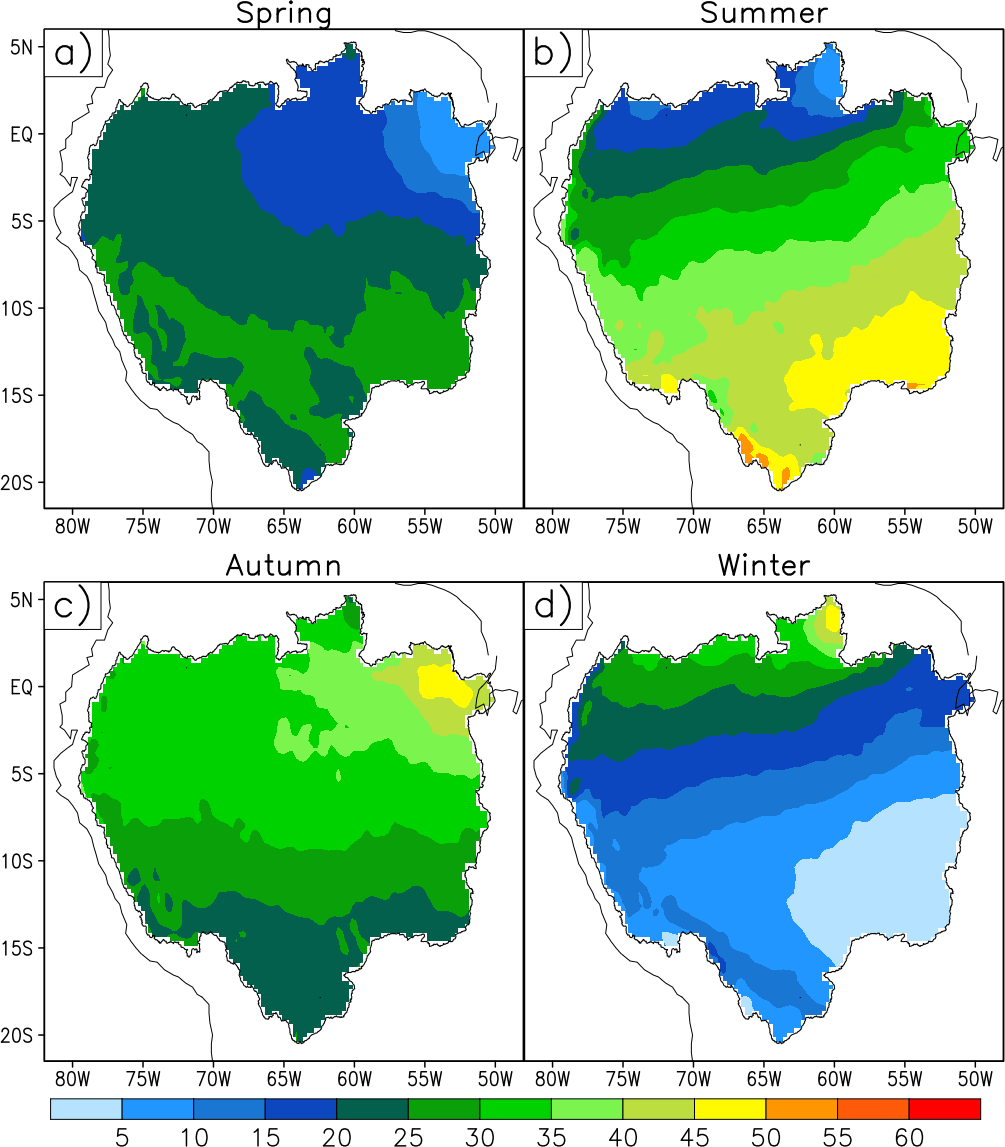
\includegraphics[width=0.55\textwidth]{pre-amz.png}
\caption{Contribución de la precipitación estacional (\%) sobre la cuenca Amazónica para el periodo 1981-2010, realizado con datos de reanálisis ERA5.}
%\raggedright Fuente: Adaptado de \cite{greenwade93}.
\label{fig01}
\end{figure}


Ahora se muestra una opción de como citar varios trabajos de investigación. Muchos estudios de modelado muestran una reducción de la precipitación y un aumento de la temperatura en la región tropical en el futuro, siendo que estos cambios son mas intensos en el escenario más pesimista (RCP8.5)~\citep{reboita14,reboita21,blazquez20,llopart20}.

Otra forma de de insertar Figuras en el contenido del documento es cuando se toma como referencia una figura de un trabajo de investigación anterior. La Figura~\ref{fig02} muestra el dominio de simulación realizado con el modelo regional. La Figura~\ref{fig03} muestra otra alternativa de citar adecuadamente la figura de otros autores. 

\begin{figure}[htbp]
\centering
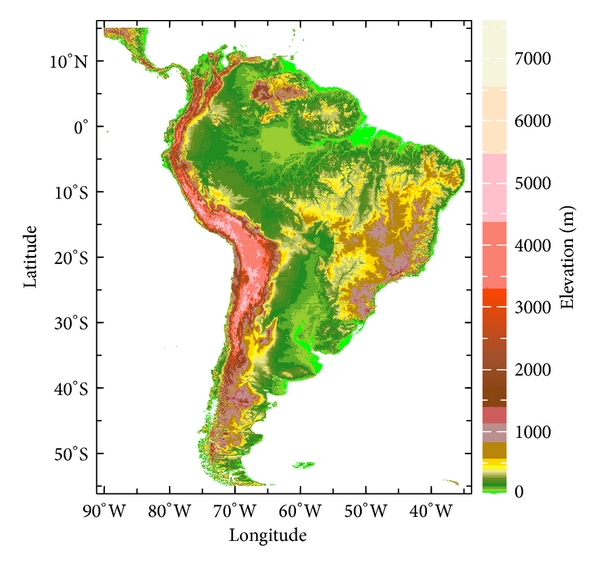
\includegraphics[width=0.8\textwidth]{topografia.jpg}
%\raggedright \textbf{Fuente:} Adaptado de \cite{solman2013}.
%\centering \textbf{Fuente:} .
\captionsource{Topografía (m) de América del Sur, generado con datos de ETOPO5.}{Obtenido de \cite{solman2013}.}
\label{fig02}
\end{figure}


\begin{figure}[!ht]
\centering
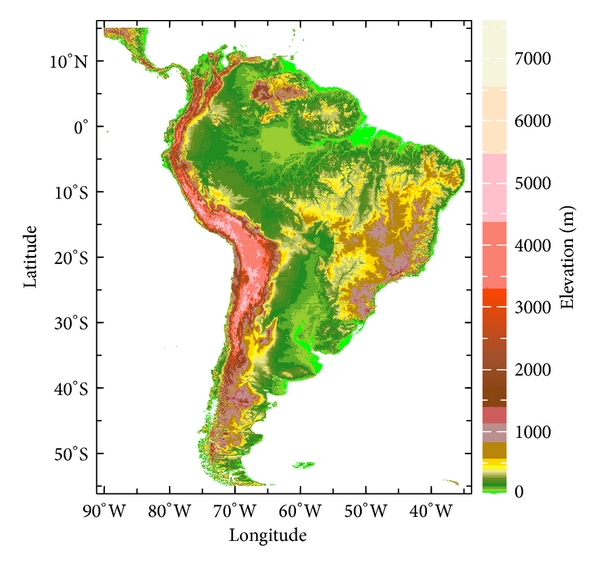
\includegraphics[width=1.0\textwidth]{topografia.jpg}
\vspace{-1.0cm}
\caption{Topografía de América del Sur.}
%\raggedright \textbf{Fuente:} Adaptado de \cite{solman2013}
\centering \textbf{Fuente:} Adaptado de \cite{solman2013}.
\label{fig03}
\end{figure}

La ecuación \(x^2 + y^2 = z^2\) muestra el teorema de Pitágoras. Otra forma de escribir ecuaciones en intermedio de los párrafos es de la siguiente manera: $(a+b)^2 = a^2 + 2ab + b^2$. La ecuación~\ref{eq1} muestra el resultado del calculo de la integral cerrada. 

\begin{equation}
\oint_{a}^{b} = \sqrt{x^2+1}
\label{eq1}
\end{equation}

También se puede insertar ecuaciones a lo largo del texto sin numeración, para ello solo debe seguir el procedimiento del siguiente ejemplo:\newline

\begin{equation*}
\oint_{a}^{b} = \sqrt{x^2+1}
\label{eq2}
\end{equation*}

Como se observa la ecuación inmediata superior no tiene la numeración. A continuación se muestra algunas alternativas de como el usuario puede centrar las ecuaciones con múltiples lineas. 

\begin{gather}
((a+b)^2 = a^2 + 2ab + b^2\\
(a-b)^2 = a^2 - 2ab + b^2\\
(a+b)(a-b) = a^2 - b^2
\end{gather}

\begin{align}
((a+b)^2& = a^2 + 2ab + b^2\\
(a-b)^2& = a^2 - 2ab + b^2\\
(a+b)(a-b)& = a^2 - b^2
\end{align}


Las Tablas también sarán insertadas a lo largo del texto, para ello ver los siguientes ejemplos:\newline


\begin{table}[!h]
\begin{center}
\begin{tabular}{| l | c | c | c | c | }
\hline
\multicolumn{5}{ |c| }{Valores promedios de precipitación} \\ \hline
\textbf{Ciudades} & \textbf{Verano} & \textbf{Otoño} & \textbf{Invierno} & \textbf{Primavera} \\ \hline
Huancayo & 80 mm & 70 mm & 10 mm & 35 mm \\
La Mar & 85 mm & 65 mm & 5 mm & 93 mm \\
Coricancha & 35 mm & 30 mm & 2 mm & 45 mm \\
Sucre & 65 mm & 45 mm & 10 mm & 20 mm \\ \hline
\end{tabular}
\caption{Valores de precipitación para tres ciudades del Perú en escala estacional durante el periodo 2000-2010.}
\label{tabla1}
\end{center}
\end{table}


La Tabla~\ref{tabla2} muestra la precipitación acumulada para las principales estaciones meteorológicas del sur de Lima. En esta tabla se puede observar que la estación 4 recibe la mínima precipitación. 

Lorem ipsum dolor sit amet, consectetur adipiscing elit. Aliquam ultricies lacinia euismod. Nam tempus risus in dolor rhoncus in interdum enim tincidunt. Donec vel nunc neque. In condimentum ullamcorper quam non consequat. Fusce sagittis tempor feugiat. Fusce magna erat, molestie eu convallis ut, tempus sed arcu. Quisque molestie, ante a tincidunt ullamcorper, sapien enim dignissim lacus, in semper nibh erat lobortis purus. Integer dapibus ligula ac risus convallis pellentesque.

\begin{table}[!h]
\centering
\begin{tabular}{|c|c|c|c|c|}
\hline
\textbf{Estación 1} & \textbf{Estación 2} & \textbf{Estación 3} & \textbf{Estación 4} & \textbf{Estación 5} \\ \hline
20    & 25     & 22     & 16     & 87      \\ \hline
30    & 45     & 65     & 22     & 57      \\ \hline
10    & 12     & 60     & 1      & 12      \\ \hline
\end{tabular}
\caption{Datos de precipitación acumulado (mm) para cinco estaciones meteorológicas.}
\label{tabla2}
\end{table}

Lorem ipsum dolor sit amet, consectetur adipiscing elit. Aliquam ultricies lacinia euismod. Nam tempus risus in dolor rhoncus in interdum enim tincidunt. Donec vel nunc neque. In condimentum ullamcorper quam non consequat. Fusce sagittis tempor feugiat. Fusce magna erat, molestie eu convallis ut, tempus sed arcu. Quisque molestie, ante a tincidunt ullamcorper, sapien enim dignissim lacus, in semper nibh erat lobortis purus. Integer dapibus ligula ac risus convallis pellentesque. Lorem ipsum dolor sit amet, consectetur adipiscing elit. Aliquam ultricies lacinia euismod. Nam tempus risus in dolor rhoncus in interdum enim tincidunt. Donec vel nunc neque. In condimentum ullamcorper quam non consequat. Fusce sagittis tempor feugiat. Fusce magna erat, molestie eu convallis ut, tempus sed arcu. Quisque molestie, ante a tincidunt ullamcorper, sapien enim dignissim lacus, in semper nibh erat lobortis purus. Integer dapibus ligula ac risus convallis pellentesque.

Lorem ipsum dolor sit amet, consectetur adipiscing elit. Aliquam ultricies lacinia euismod. Nam tempus risus in dolor rhoncus in interdum enim tincidunt. Donec vel nunc neque. In condimentum ullamcorper quam non consequat. Fusce sagittis tempor feugiat. Fusce magna erat, molestie eu convallis ut, tempus sed arcu. Quisque molestie, ante a tincidunt ullamcorper, sapien enim dignissim lacus, in semper nibh erat lobortis purus. Integer dapibus ligula ac risus convallis pellentesque. Lorem ipsum dolor sit amet, consectetur adipiscing elit. Aliquam ultricies lacinia euismod. Nam tempus risus in dolor rhoncus in interdum enim tincidunt. Donec vel nunc neque. In condimentum ullamcorper quam non consequat. Fusce sagittis tempor feugiat. Fusce magna erat, molestie eu convallis ut, tempus sed arcu. Quisque molestie, ante a tincidunt ullamcorper, sapien enim dignissim lacus, in semper nibh erat lobortis purus. Integer dapibus ligula ac risus convallis pellentesque. 

\section{Motivación}
Escriba aquí la motivación de su trabajo de investigación si lo tuviera ....


\section{Objetivo}
Escriba aquí el objetivo de su trabajo de investigación... 

\subsection{Objetivos específicos}
Escriba aquí sus objetivos de su investigación si los tuviera.... 
 %% 1o capítulo
%=============================
%  SEGUNDO CAPITULO
%=============================
\chapter{Marco Teórico}
\label{cap2}

En este capitulo tiene que describir el fundamento teórico de su investigación. Esto ayudara al lector a entender mas fácil el trabajo que ira a desarrollar. De forma general, usted tiene que estructurar todo el contenido de su investigación de la mejor forma posible para que el lector pueda entender su trabajo de investigación. 

\section{Área de estudio}
Colocar el texto correspondiente... %% 2o capítulo
%=============================
%  TERCER CAPITULO
%=============================
\chapter{Datos y Metodología}
\label{cap3}

En esta sección escribir los datos utilizados en su investigación, así como la metodología.


\section{Datos observados}
Colocar el texto correspondiente ...

\section{Metodología}

Colocar el texto correspondiente ...
 %% 3o capítulo
%=============================
%  CUARTO CAPITULO
%=============================
\chapter{Resultados}
\label{cap4}


En este capitulo escribir el resultado de su investigación científica.

A continuación se muestra algunas secciones en los que puede dividir los resultados de su investigación.

\section{Análisis Estacional de las precipitaciones}

Lorem ipsum dolor sit amet, consectetur adipiscing elit. Aliquam ultricies lacinia euismod. Nam tempus risus in dolor rhoncus in interdum enim tincidunt. Donec vel nunc neque. In condimentum ullamcorper quam non consequat. Fusce sagittis tempor feugiat. Fusce magna erat, molestie eu convallis ut, tempus sed arcu. Quisque molestie, ante a tincidunt ullamcorper, sapien enim dignissim lacus, in semper nibh erat lobortis purus. Integer dapibus ligula ac risus convallis pellentesque. Lorem ipsum dolor sit amet, consectetur adipiscing elit. Aliquam ultricies lacinia euismod. Nam tempus risus in dolor rhoncus in interdum enim tincidunt. Donec vel nunc neque. In condimentum ullamcorper quam non consequat. Fusce sagittis tempor feugiat. Fusce magna erat, molestie eu convallis ut, tempus sed arcu. Quisque molestie, ante a tincidunt ullamcorper, sapien enim dignissim lacus, in semper nibh erat lobortis purus. Integer dapibus ligula ac risus convallis pellentesque.

\section{Análisis estacional de la temperatura de superficie del mar}


A continuación se muestra algunas alternativas de como hacer colocar la leyenda a las figuras, así como su respectiva fuente. Para mayor detalle observe detalladamente las figuras. La Figura \ref{fig-enso} muestra la influencia del ENSO en las tasas de precipitación que ocurren sobre América del Sur. 


\begin{figure}[H]
\centering
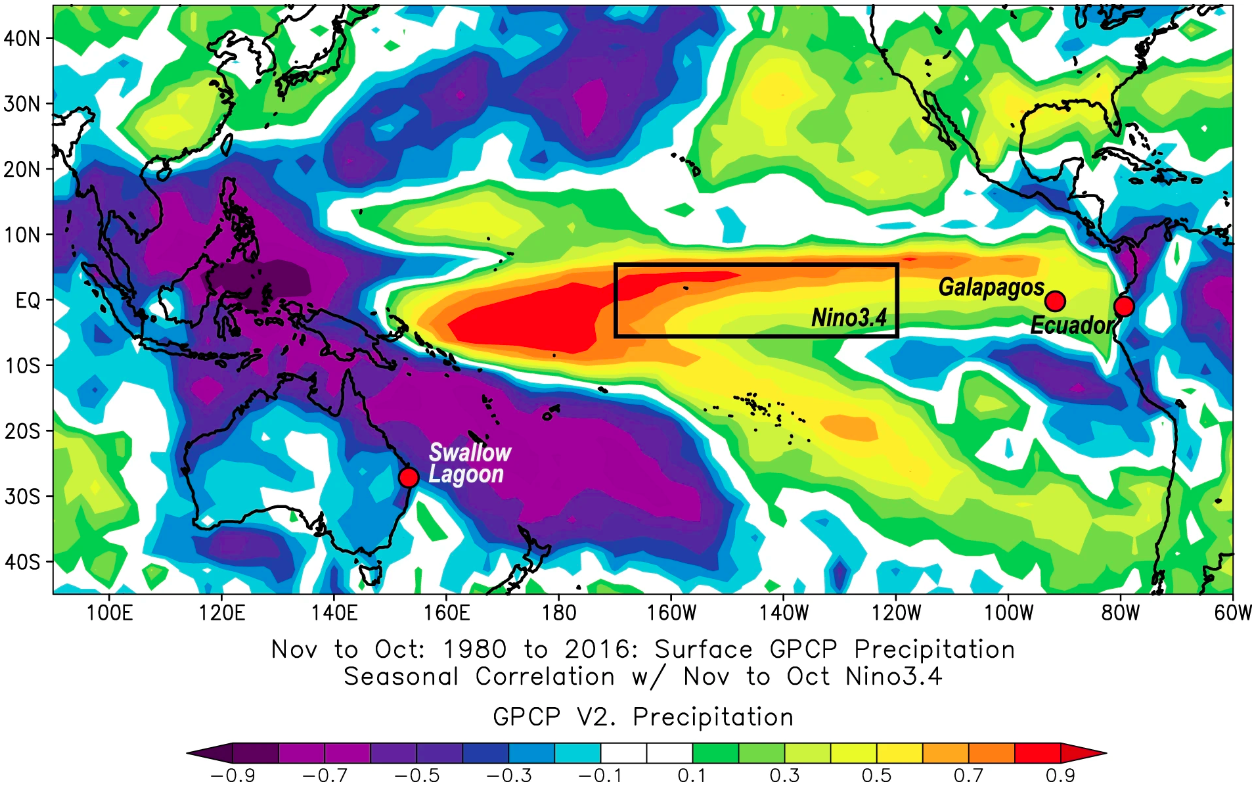
\includegraphics[width=1.0\textwidth]{Figuras/enso.png}
\vspace{-0.5cm}
\caption{Influencia del ENSO en la precipitación de América del Sur.}
\textbf{Fuente:} Adaptado de \cite{barr2019}.
\label{fig-enso}
\end{figure}

Segunda alternativa de colocar la leyenda y la fuente se muestra en la Figura~\ref{fig-enso2}:


\begin{figure}[H]
\centering
\caption{Influencia del ENSO en la precipitación de América del Sur.}
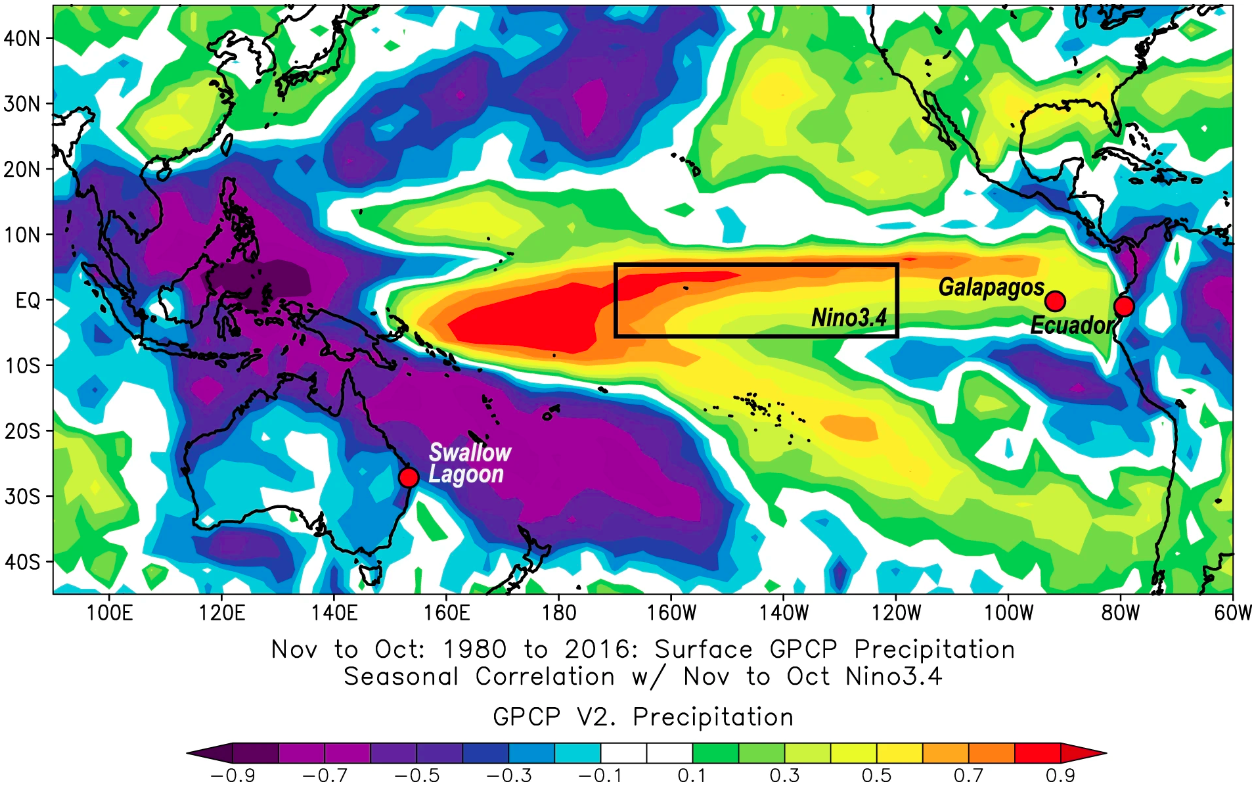
\includegraphics[width=1.0\textwidth]{Figuras/enso.png}
\vspace{-0.5cm}
\textbf{Fuente:} Adaptado de \cite{barr2019}.
\label{fig-enso2}
\end{figure}

Tercera alternativa de colocar la leyenda y la fuente se muestra en la Figura~\ref{fig-enso3}:

\begin{figure}[H]
\centering
\caption{Influencia del ENSO en la precipitación de América del Sur.}
\copyrightbox[b]{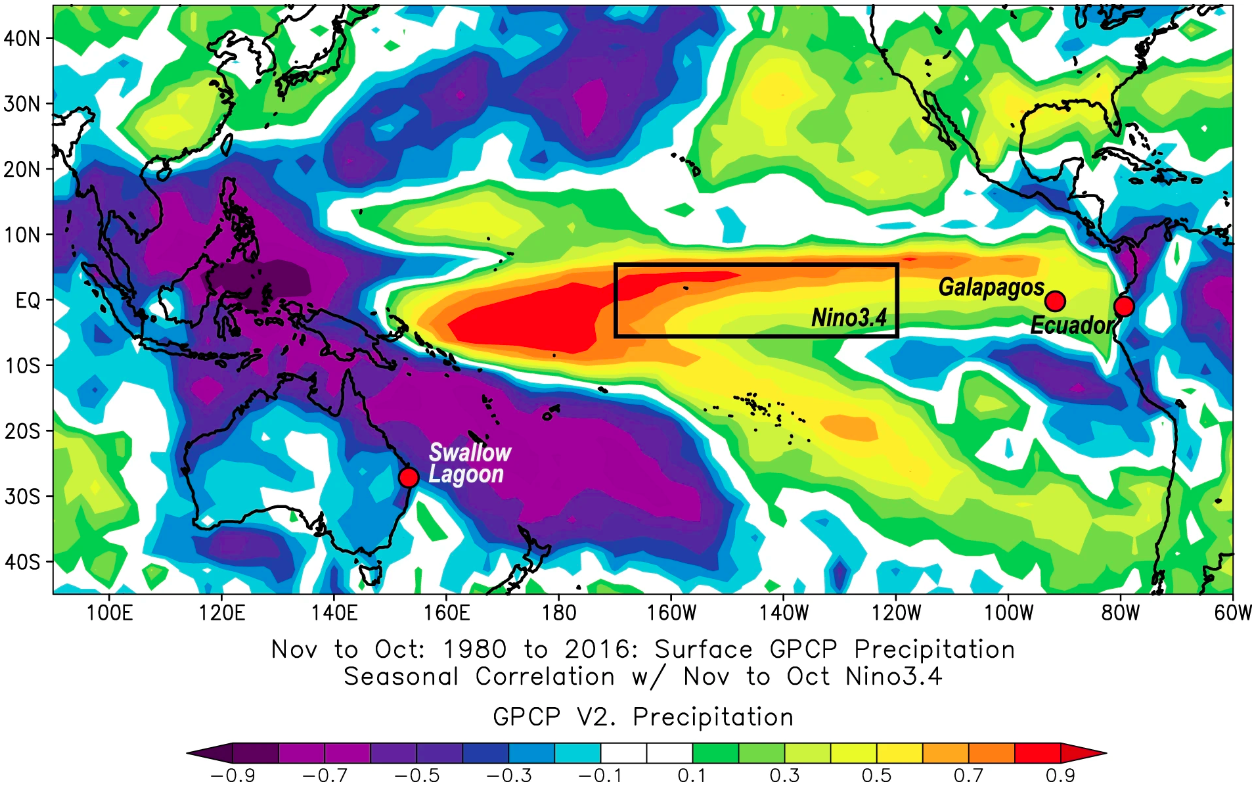
\includegraphics[width=1.0\linewidth]{Figuras/enso.png}}%
                {Fuente: Adaptado de \cite{barr2019}.}
\label{fig-enso3}
\end{figure} %% 4o capítulo
%\include{./Docs/cap5} %% 5o capítulo
%\include{./Docs/cap6} %% 6o capítulo
%\include{./Docs/cap7} %% 7o capítulo

\newpage
%===========================
%  REFERENCIA  BIBLIOGRAFÍA
%===========================
\bibliographystyle{./Bib/apalike-es}
\bibliography{./Bib/referencias}

%======================================
%COMENTAR SI NO DESEA QUE APAREZCA EN EL INDICE GENERAL
%========================================================
\addcontentsline{toc}{chapter}{Referencias Bibliográficas}

%==============================================================
%  SE ADICIONA LAS SECCIONES: ANEXO Y APÉNDICE 
%
%  COMENTAR SI NO DESEA QUE APAREZCA ESTA PARTE DEL DOCUMENTO
%==============================================================
\appendix{}
\renewcommand{\appendixname}{Anexos}
\renewcommand{\appendixtocname}{Anexos}
\renewcommand{\appendixpagename}{Anexos}
\clearpage
\addappheadtotoc
\appendixpage

%==========================================
%\setcounter{figure}{0}
%\numberwithin{figure}{chapter}
%\numberwithin{table}{section}
%==========================================

%========================= ANEXO 1 ===========================
\chapter{Anexo I: Características de las nubes}
\label{anexoI}

Colocar aquí la información correspondiente.



%========================= ANEXO 2 ===========================
%\chapter{Anexo II: Tablas de doble entrada para el análisis de datos geofísicos}
%\label{anexoII}

%Colocar aquí la información correspondiente. %% Opcional
%==========================================
%\setcounter{figure}{0}
%\numberwithin{figure}{chapter}
%\numberwithin{table}{section}
%==========================================
\appendix{}
\renewcommand{\appendixname}{Apéndices}
\renewcommand{\appendixtocname}{Apéndices}
\renewcommand{\appendixpagename}{Apéndices}
\clearpage
\addappheadtotoc
\appendixpage

%========================= APÉNDICE 1 ===========================
\chapter{Apéndice I: Índice de secas y inundaciones}
\label{apendiceI}

Colocar aquí la información correspondiente.



%========================= APÉNDICE 2 ===========================
%\chapter{Apéndice II: Tablas de doble entrada para el análisis de datos geofísicos}
%\label{apendiceII}

%Colocar aquí la información correspondiente.

 %% Opcional

\end{document}